\documentclass[aspectratio=169,12pt]{beamer}

% ── NeurIPS color scheme ──
\usepackage{xcolor}
\definecolor{primary}{HTML}{8B5CF6}
\definecolor{accent}{HTML}{2563EB}
\definecolor{darktext}{HTML}{1E1E1E}
\definecolor{lightbg}{HTML}{F8F9FA}
\definecolor{dangerred}{HTML}{DC2626}
\definecolor{safegreen}{HTML}{059669}

% ── Clean theme ──
\usetheme{default}
\usecolortheme{default}
\setbeamercolor{frametitle}{fg=primary}
\setbeamercolor{title}{fg=primary}
\setbeamercolor{structure}{fg=accent}
\setbeamercolor{itemize item}{fg=primary}
\setbeamercolor{itemize subitem}{fg=accent}
\setbeamercolor{alerted text}{fg=dangerred}
\setbeamertemplate{navigation symbols}{}
\setbeamertemplate{footline}{
  \hfill\usebeamercolor[fg]{frametitle}\insertframenumber/\inserttotalframenumber\hspace{4mm}\vspace{2mm}
}
\setbeamerfont{frametitle}{series=\bfseries,size=\Large}
\setbeamerfont{title}{series=\bfseries,size=\huge}

% ── Packages ──
\usepackage{graphicx,amsmath,amssymb,booktabs,tikz,pgfplots}
\usepackage{fontenc}
\usetikzlibrary{arrows.meta,positioning,shapes,calc,decorations.pathreplacing}
\pgfplotsset{compat=1.18}

% ── Metadata ──
\title{RDSA: Resilient Distributed\\Safety Architecture}
\subtitle{Defending VLMs Against Adversarial Safety Attacks\\via Distributed, Entangled Safety Representations}
\author{Tianhao}
\institute{University of Virginia}
\date{Milestone Report --- March 2026}

\begin{document}

% ═══════════════════════════════════════════════════════════════
% Slide 1: Title
% ═══════════════════════════════════════════════════════════════
\begin{frame}[plain]
\titlepage
\end{frame}

% ═══════════════════════════════════════════════════════════════
% Slide 2: Outline
% ═══════════════════════════════════════════════════════════════
\begin{frame}{Outline}
\begin{enumerate}
  \item \textbf{Problem}: VLM safety is fragile --- one attack breaks it
  \item \textbf{Root cause}: Safety features are localized \& separable
  \item \textbf{Our approach}: RDSA --- distribute, entangle, harden
  \item \textbf{Technical details}: Three defense modules + theory
  \item \textbf{Progress}: Implementation \& preliminary results
  \item \textbf{Timeline}: Path to NeurIPS 2026
\end{enumerate}
\end{frame}

% ═══════════════════════════════════════════════════════════════
% Slide 3: The Problem
% ═══════════════════════════════════════════════════════════════
\begin{frame}{VLM Safety Is Surprisingly Fragile}
\begin{columns}[T]
\begin{column}{0.55\textwidth}
\begin{itemize}
  \item VLMs (GPT-4o, Qwen-VL, Gemma) have safety alignment
  \item \alert{One adversarial image can bypass all safety guardrails}
  \item SCIA attack (ICML 2026): \textbf{>80\% ASR} on aligned models
  \item Safety fine-tuning, RLHF --- all broken by visual attacks
\end{itemize}
\vspace{1em}
\textbf{Why?} $\rightarrow$ Next slide
\end{column}
\begin{column}{0.42\textwidth}
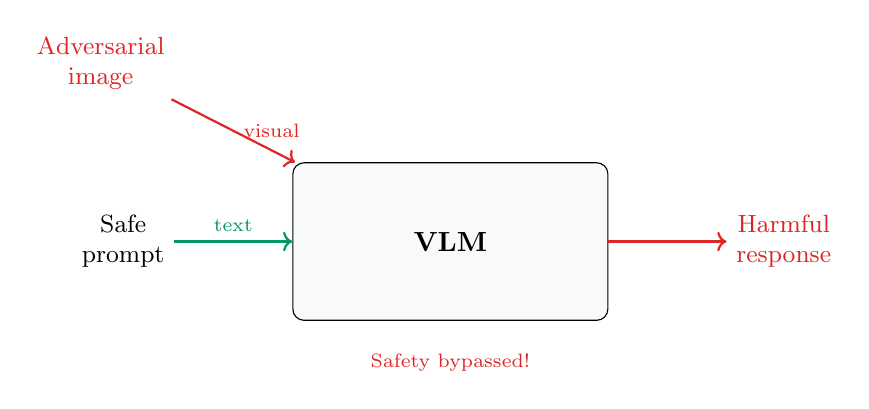
\begin{tikzpicture}[scale=0.7]
  % VLM box
  \node[draw,rounded corners,fill=lightbg,minimum width=4cm,minimum height=2cm] (vlm) at (0,0) {\textbf{VLM}};
  % Safe input
  \node[left=1.5cm of vlm,align=center,font=\small] (safe) {Safe\\prompt};
  \draw[->,thick,safegreen] (safe) -- (vlm) node[midway,above,font=\scriptsize] {text};
  % Adversarial image
  \node[above left=0.8cm and 1.5cm of vlm,align=center,font=\small,text=dangerred] (adv) {Adversarial\\image};
  \draw[->,thick,dangerred] (adv) -- (vlm) node[midway,right,font=\scriptsize] {visual};
  % Output
  \node[right=1.5cm of vlm,align=center,font=\small,text=dangerred] (out) {Harmful\\response};
  \draw[->,thick,dangerred] (vlm) -- (out);
  % Cross on safety
  \node[below=0.3cm of vlm,font=\scriptsize,text=dangerred] {Safety bypassed!};
\end{tikzpicture}
\end{column}
\end{columns}
\end{frame}

% ═══════════════════════════════════════════════════════════════
% Slide 4: Root Cause (SCIA Finding)
% ═══════════════════════════════════════════════════════════════
\begin{frame}{Root Cause: Localized \& Separable Safety Features}
\begin{columns}[T]
\begin{column}{0.55\textwidth}
SCIA's key discovery:
\begin{itemize}
  \item Safety behavior depends on \textbf{$\sim$0.1--0.5\%} of neurons
  \item These neurons are \alert{disentangled from semantics}
  \item Attacker can suppress safety \textbf{without hurting capability}
\end{itemize}
\vspace{0.8em}
\textcolor{accent}{\textbf{Analogy:}} Safety is a single fuse ---\\cut it, lights stay on, alarm goes off
\end{column}
\begin{column}{0.42\textwidth}
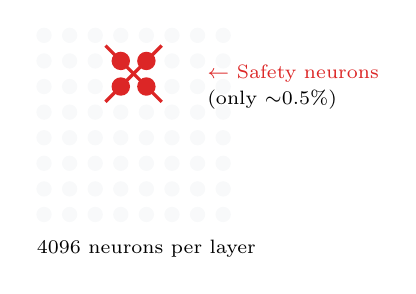
\begin{tikzpicture}[scale=0.65]
  % Grid of neurons
  \foreach \x in {0,...,7} {
    \foreach \y in {0,...,7} {
      \fill[lightbg] (\x*0.5, \y*0.5) circle (0.15);
    }
  }
  % Safety neurons (few, clustered)
  \fill[dangerred] (1.5,2.5) circle (0.18);
  \fill[dangerred] (2.0,2.5) circle (0.18);
  \fill[dangerred] (1.5,3.0) circle (0.18);
  \fill[dangerred] (2.0,3.0) circle (0.18);
  % Labels
  \node[font=\scriptsize,below] at (2,-0.3) {4096 neurons per layer};
  \node[font=\scriptsize,dangerred,right] at (3.0,2.75) {$\leftarrow$ Safety neurons};
  \node[font=\scriptsize,right] at (3.0,2.25) {(only $\sim$0.5\%)};
  % Strike through
  \draw[dangerred,very thick] (1.2,2.2) -- (2.3,3.3);
  \draw[dangerred,very thick] (2.3,2.2) -- (1.2,3.3);
\end{tikzpicture}
\end{column}
\end{columns}
\end{frame}

% ═══════════════════════════════════════════════════════════════
% Slide 5: Our Key Insight
% ═══════════════════════════════════════════════════════════════
\begin{frame}{Key Insight: Distribute, Entangle, Harden}
\centering
\vspace{0.5em}
{\Large\textcolor{primary}{\textbf{Make safety features impossible to remove\\without destroying the model}}}
\vspace{1.5em}

\begin{columns}[c]
\begin{column}{0.32\textwidth}
\centering
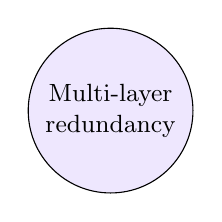
\begin{tikzpicture}
  \node[draw,circle,fill=primary!15,minimum size=1.5cm,font=\small,align=center] {Multi-layer\\redundancy};
\end{tikzpicture}\\[0.5em]
{\small\textbf{Distribute} safety\\across layer groups}
\end{column}
\begin{column}{0.32\textwidth}
\centering
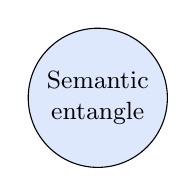
\begin{tikzpicture}
  \node[draw,circle,fill=accent!15,minimum size=1.5cm,font=\small,align=center] {Semantic\\entangle};
\end{tikzpicture}\\[0.5em]
{\small\textbf{Entangle} safety\\with semantics}
\end{column}
\begin{column}{0.32\textwidth}
\centering
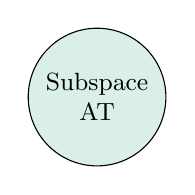
\begin{tikzpicture}
  \node[draw,circle,fill=safegreen!15,minimum size=1.5cm,font=\small,align=center] {Subspace\\AT};
\end{tikzpicture}\\[0.5em]
{\small\textbf{Harden} via\\adversarial training}
\end{column}
\end{columns}
\end{frame}

% ═══════════════════════════════════════════════════════════════
% Slide 6: RDSA Architecture Overview
% ═══════════════════════════════════════════════════════════════
\begin{frame}{RDSA: Three Defense Modules}
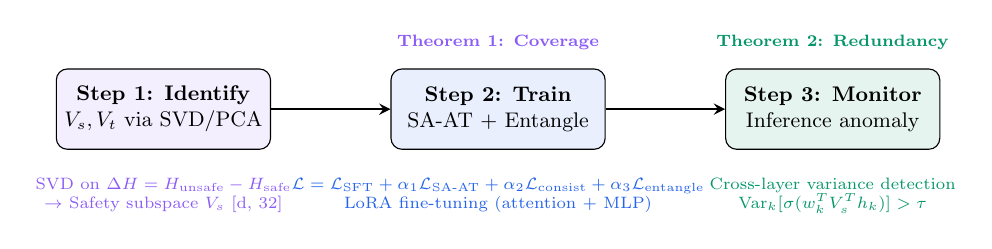
\begin{tikzpicture}[
  box/.style={draw,rounded corners,minimum width=3.2cm,minimum height=1.2cm,align=center,font=\small},
  arrow/.style={->,>=stealth,thick},
  scale=0.85, transform shape
]
  % Pipeline
  \node[box,fill=primary!10] (id) at (0,0) {\textbf{Step 1: Identify}\\$V_s, V_t$ via SVD/PCA};
  \node[box,fill=accent!10] (train) at (5,0) {\textbf{Step 2: Train}\\SA-AT + Entangle};
  \node[box,fill=safegreen!10] (monitor) at (10,0) {\textbf{Step 3: Monitor}\\Inference anomaly};

  \draw[arrow] (id) -- (train);
  \draw[arrow] (train) -- (monitor);

  % Details below
  \node[font=\scriptsize,text=primary,below=0.3cm of id,align=center] {
    SVD on $\Delta H = H_\text{unsafe} - H_\text{safe}$\\
    $\rightarrow$ Safety subspace $V_s$ [d, 32]
  };
  \node[font=\scriptsize,text=accent,below=0.3cm of train,align=center] {
    $\mathcal{L} = \mathcal{L}_\text{SFT} + \alpha_1 \mathcal{L}_\text{SA-AT} + \alpha_2 \mathcal{L}_\text{consist} + \alpha_3 \mathcal{L}_\text{entangle}$\\
    LoRA fine-tuning (attention + MLP)
  };
  \node[font=\scriptsize,text=safegreen,below=0.3cm of monitor,align=center] {
    Cross-layer variance detection\\
    $\text{Var}_k[\sigma(w_k^T V_s^T h_k)] > \tau$
  };

  % Theorem annotations
  \node[font=\scriptsize,primary,above=0.15cm of train] {\textbf{Theorem 1: Coverage}};
  \node[font=\scriptsize,safegreen,above=0.15cm of monitor] {\textbf{Theorem 2: Redundancy}};
\end{tikzpicture}
\end{frame}

% ═══════════════════════════════════════════════════════════════
% Slide 7: Module 1 — SA-AT (Theorem 1)
% ═══════════════════════════════════════════════════════════════
\begin{frame}{Module 1: Subspace-Constrained Adversarial Training}
\textbf{Theorem 1} (SA-AT Coverage Guarantee):
\vspace{0.3em}
\begin{itemize}
  \item \textbf{Inner loop}: PGD finds worst-case $\delta^*$ in $V_s$ subspace
  $$\delta^* = \arg\max_{\|\delta\| \leq \varepsilon} \mathcal{L}_\text{CE}\big(f(h + V_s\delta),\; y_\text{refusal}\big)$$
  \item \textbf{Outer loop}: Train model to refuse under $\delta^*$
  \item Search space is only \textbf{$d_s$=32 dimensions} (not 4096)
  \item \textcolor{accent}{Random restarts} (3$\times$) for stronger adversarial search
  \item \textcolor{accent}{Relative $\varepsilon$}: scaled by activation norm per layer
\end{itemize}
\end{frame}

% ═══════════════════════════════════════════════════════════════
% Slide 8: Module 2 — Cross-Layer Redundancy (Theorem 2)
% ═══════════════════════════════════════════════════════════════
\begin{frame}{Module 2: Cross-Layer Safety Redundancy}
\textbf{Theorem 2}: Attack cost amplification via $G$ independent layer groups

\vspace{0.5em}
\begin{columns}[T]
\begin{column}{0.52\textwidth}
\begin{itemize}
  \item Safety distributed across \textbf{$G$=3 groups}
  \item Attack cost: $O(\varepsilon_1^*) \rightarrow O\!\left(\sqrt{\textstyle\sum_k (\varepsilon_k^*)^2}\right)$
  \item Attacker must fool \textbf{all groups simultaneously}
  \item Non-aligned gradients across groups
\end{itemize}
\end{column}
\begin{column}{0.45\textwidth}
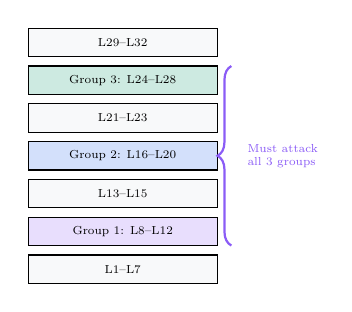
\begin{tikzpicture}[scale=0.6, transform shape]
  % Layer stack
  \foreach \i/\label in {0/L1--L7, 1/L8--L12, 2/L13--L15, 3/L16--L20, 4/L21--L23, 5/L24--L28, 6/L29--L32} {
    \pgfmathsetmacro{\ypos}{\i*0.8}
    \ifnum\i=1
      \node[draw,fill=primary!20,minimum width=4cm,minimum height=0.6cm,font=\scriptsize] at (0,\ypos) {Group 1: \label};
    \else\ifnum\i=3
      \node[draw,fill=accent!20,minimum width=4cm,minimum height=0.6cm,font=\scriptsize] at (0,\ypos) {Group 2: \label};
    \else\ifnum\i=5
      \node[draw,fill=safegreen!20,minimum width=4cm,minimum height=0.6cm,font=\scriptsize] at (0,\ypos) {Group 3: \label};
    \else
      \node[draw,fill=lightbg,minimum width=4cm,minimum height=0.6cm,font=\scriptsize] at (0,\ypos) {\label};
    \fi\fi\fi
  }
  % Brace
  \draw[decorate,decoration={brace,amplitude=5pt},thick,primary] (2.3,0.5) -- (2.3,4.3) node[midway,right=6pt,font=\scriptsize,align=left] {Must attack\\all 3 groups};
\end{tikzpicture}
\end{column}
\end{columns}
\end{frame}

% ═══════════════════════════════════════════════════════════════
% Slide 9: Module 3 — Entanglement
% ═══════════════════════════════════════════════════════════════
\begin{frame}{Module 3: Safety-Semantic Entanglement}
\begin{columns}[T]
\begin{column}{0.55\textwidth}
\textbf{Goal}: Make safety inseparable from semantics
\vspace{0.5em}
\begin{itemize}
  \item Entanglement degree: $\eta = \frac{1}{d_s}\sum_i \max_j |v_s^{(i)\top} v_t^{(j)}|$
  \item $\eta \approx 0$ $\rightarrow$ safety removable (vulnerable)
  \item $\eta \approx 1$ $\rightarrow$ safety = semantics (robust)
  \item \textbf{New}: $\mathcal{L}_\text{entangle} = 1 - \eta$
  \item Directly optimized via gradient descent
\end{itemize}
\vspace{0.5em}
\textcolor{accent}{Attacker's dilemma}: removing safety\\destroys model capability
\end{column}
\begin{column}{0.42\textwidth}
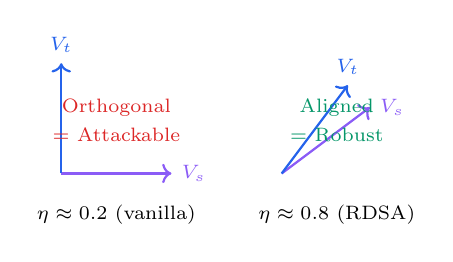
\begin{tikzpicture}[scale=0.7]
  % Low eta
  \begin{scope}[shift={(0,3)}]
    \draw[primary,thick,->] (0,0) -- (2,0) node[right,font=\scriptsize] {$V_s$};
    \draw[accent,thick,->] (0,0) -- (0,2) node[above,font=\scriptsize] {$V_t$};
    \node[font=\scriptsize,below] at (1,-0.4) {$\eta \approx 0.2$ (vanilla)};
    \node[font=\scriptsize,dangerred] at (1,1.2) {Orthogonal};
    \node[font=\scriptsize,dangerred] at (1,0.7) {= Attackable};
  \end{scope}
  % High eta
  \begin{scope}[shift={(4,3)}]
    \draw[primary,thick,->] (0,0) -- (1.6,1.2) node[right,font=\scriptsize] {$V_s$};
    \draw[accent,thick,->] (0,0) -- (1.2,1.6) node[above,font=\scriptsize] {$V_t$};
    \node[font=\scriptsize,below] at (1,-0.4) {$\eta \approx 0.8$ (RDSA)};
    \node[font=\scriptsize,safegreen] at (1,1.2) {Aligned};
    \node[font=\scriptsize,safegreen] at (1,0.7) {= Robust};
  \end{scope}
\end{tikzpicture}
\end{column}
\end{columns}
\end{frame}

% ═══════════════════════════════════════════════════════════════
% Slide 10: Training Pipeline
% ═══════════════════════════════════════════════════════════════
\begin{frame}{Training Pipeline: 10 Key Enhancements}
\begin{columns}[T]
\begin{column}{0.48\textwidth}
\textbf{Data \& Format}
\begin{itemize}
  \item[\textcolor{safegreen}{\checkmark}] Chat template formatting
  \item[\textcolor{safegreen}{\checkmark}] Label masking (response only)
  \item[\textcolor{safegreen}{\checkmark}] LoRA: attention + MLP modules
\end{itemize}
\vspace{0.5em}
\textbf{SA-AT Improvements}
\begin{itemize}
  \item[\textcolor{safegreen}{\checkmark}] PGD random restarts ($3\times$)
  \item[\textcolor{safegreen}{\checkmark}] Relative $\varepsilon$ (5\% of $\|h\|$)
  \item[\textcolor{safegreen}{\checkmark}] Warmup: 1 epoch pure SFT first
\end{itemize}
\end{column}
\begin{column}{0.48\textwidth}
\textbf{New Losses}
\begin{itemize}
  \item[\textcolor{safegreen}{\checkmark}] $\mathcal{L}_\text{entangle}$: optimize $\eta$ directly
  \item[\textcolor{safegreen}{\checkmark}] $\mathcal{L}_\text{consist}$: harmful samples only
\end{itemize}
\vspace{0.5em}
\textbf{Robustness}
\begin{itemize}
  \item[\textcolor{safegreen}{\checkmark}] Multi-layer hooks (all group layers)
  \item[\textcolor{safegreen}{\checkmark}] Intra-epoch subspace refresh
\end{itemize}
\end{column}
\end{columns}
\end{frame}

% ═══════════════════════════════════════════════════════════════
% Slide 11: Models & Evaluation
% ═══════════════════════════════════════════════════════════════
\begin{frame}{Models \& Evaluation Setup}
\begin{columns}[T]
\begin{column}{0.48\textwidth}
\textbf{Surrogate Models (white-box)}
\begin{itemize}
  \item Qwen3-VL-8B \textcolor{safegreen}{$\checkmark$}
  \item InternVL2.5-8B \textcolor{safegreen}{$\checkmark$}
  \item MiniCPM-V-2.6 \textcolor{safegreen}{$\checkmark$}
\end{itemize}
\vspace{0.5em}
\textbf{6 Attack Types}
\begin{itemize}
  \item SCIA, UMK (white-box)
  \item FigStep (visual injection)
  \item 3 adaptive attacks (knows RDSA)
\end{itemize}
\end{column}
\begin{column}{0.48\textwidth}
\textbf{Metrics}
\begin{itemize}
  \item ASR$\downarrow$ --- Attack Success Rate
  \item RR$\uparrow$ --- Refusal Rate
  \item OR$\downarrow$ --- Over-Refusal Rate
  \item VQAv2, MMBench, MME (capability)
\end{itemize}
\vspace{0.5em}
\textbf{Safety Judge}
\begin{itemize}
  \item GPT-4o as judge (OpenAI API)
  \item 3 seeds for significance
\end{itemize}
\end{column}
\end{columns}
\end{frame}

% ═══════════════════════════════════════════════════════════════
% Slide 12: Preliminary Results
% ═══════════════════════════════════════════════════════════════
\begin{frame}{Preliminary Results: Qwen3-VL-8B}
\begin{columns}[T]
\begin{column}{0.48\textwidth}
\textbf{Subspace Identification}
\begin{itemize}
  \item $V_s$: [4096, 32], $V_t$: [4096, 256]
  \item Vanilla $\eta \approx 0.49$--$0.53$
  \item 3 layer groups identified
  \item Singular values: 333 $\rightarrow$ 7478 (deep layers)
\end{itemize}
\vspace{0.5em}
\textbf{Baseline (no attack)}
\begin{itemize}
  \item Vanilla ASR $\approx$ \textbf{21.6\%}
  \item Vanilla RR $\approx$ \textbf{78.4\%}
\end{itemize}
\end{column}
\begin{column}{0.48\textwidth}
\textbf{Training Status}
\begin{itemize}
  \item SA-AT warmup epoch: running
  \item Consistency loss: $0.63 \rightarrow 0.02$
  \item Entanglement loss: $0.96 \rightarrow 0.92$
  \item SFT loss: converging
\end{itemize}
\vspace{0.5em}
\textbf{Expected After Training}
\begin{itemize}
  \item ASR $< 10\%$ under SCIA
  \item ASR $< 20\%$ under adaptive
  \item VQA drop $< 2\%$
\end{itemize}
\end{column}
\end{columns}
\end{frame}

% ═══════════════════════════════════════════════════════════════
% Slide 13: Experiment Plan (10 Experiments)
% ═══════════════════════════════════════════════════════════════
\begin{frame}{NeurIPS Experiment Plan: 10 Experiments}
\small
\begin{tabular}{clll}
\toprule
\textbf{\#} & \textbf{Experiment} & \textbf{Output} & \textbf{Status} \\
\midrule
1 & Main comparison (7 def $\times$ 6 atk $\times$ 3 models) & Table 1 & In progress \\
2 & Ablation (6 variants) & Table 2 & Ready \\
3 & SA-AT analysis (PGD, $\varepsilon$, restarts) & Fig 2--3 & Ready \\
4 & Cross-layer redundancy (G=1,2,3) & Fig 4--5 & Ready \\
5 & Entanglement ($\eta$ profile, $\eta$ vs ASR) & Fig 6 & Ready \\
6 & Capability (VQAv2, MMBench, MME) & Table 4 & Ready \\
7 & Adaptive attacks (strong budget) & Table 5 & Ready \\
8 & Transfer attack (surrogate $\rightarrow$ victim) & Table 6 & Planned \\
9 & Parameter sensitivity (7 params) & Fig 7 & Ready \\
10 & Pareto frontier (safety vs utility) & Fig 1 & Planned \\
\bottomrule
\end{tabular}
\vspace{0.5em}

Total: $\sim$600 GPU-hours (1 seed) / $\sim$1800 GPU-hours (3 seeds)
\end{frame}

% ═══════════════════════════════════════════════════════════════
% Slide 14: Implementation Status
% ═══════════════════════════════════════════════════════════════
\begin{frame}{Implementation Status}
\begin{columns}[T]
\begin{column}{0.48\textwidth}
\textbf{\textcolor{safegreen}{Completed}}
\begin{itemize}
  \item[\textcolor{safegreen}{\checkmark}] Subspace identification (SVD+PCA)
  \item[\textcolor{safegreen}{\checkmark}] SA-AT training loop
  \item[\textcolor{safegreen}{\checkmark}] 4 loss functions
  \item[\textcolor{safegreen}{\checkmark}] 6 attack implementations
  \item[\textcolor{safegreen}{\checkmark}] GPT-4o safety judge
  \item[\textcolor{safegreen}{\checkmark}] 4 capability benchmarks
  \item[\textcolor{safegreen}{\checkmark}] 10 experiment scripts
  \item[\textcolor{safegreen}{\checkmark}] 3 open-access VLMs
\end{itemize}
\end{column}
\begin{column}{0.48\textwidth}
\textbf{\textcolor{accent}{In Progress}}
\begin{itemize}
  \item[$\circ$] Full RDSA training (5 epochs)
  \item[$\circ$] Evaluation with real attacks
  \item[$\circ$] Baseline defense reproduction
\end{itemize}
\vspace{0.5em}
\textbf{\textcolor{primary}{Codebase}}
\begin{itemize}
  \item $\sim$5000 lines of Python
  \item Hydra config management
  \item wandb logging
  \item Full test suite
\end{itemize}
\end{column}
\end{columns}
\end{frame}

% ═══════════════════════════════════════════════════════════════
% Slide 15: Timeline to NeurIPS
% ═══════════════════════════════════════════════════════════════
\begin{frame}{Timeline to NeurIPS 2026}
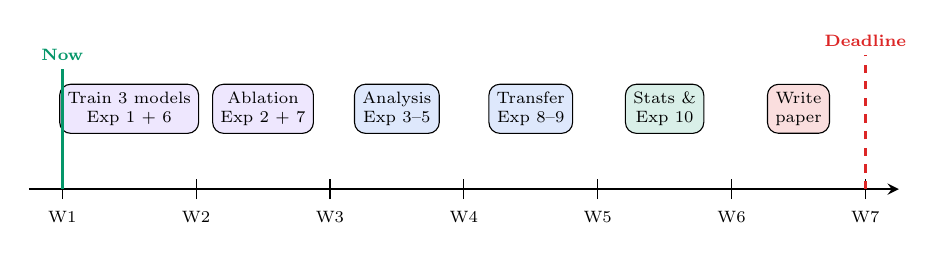
\begin{tikzpicture}[scale=0.85, transform shape]
  % Timeline
  \draw[thick,->,>=stealth] (0,0) -- (13,0);

  % Weeks
  \foreach \x/\label in {0.5/W1, 2.5/W2, 4.5/W3, 6.5/W4, 8.5/W5, 10.5/W6, 12.5/W7} {
    \draw (\x,-0.15) -- (\x,0.15);
    \node[below,font=\scriptsize] at (\x,-0.2) {\label};
  }

  % Tasks
  \node[draw,fill=primary!15,rounded corners,minimum height=0.6cm,font=\scriptsize,align=center] at (1.5,1.2) {Train 3 models\\Exp 1 + 6};
  \node[draw,fill=primary!15,rounded corners,minimum height=0.6cm,font=\scriptsize,align=center] at (3.5,1.2) {Ablation\\Exp 2 + 7};
  \node[draw,fill=accent!15,rounded corners,minimum height=0.6cm,font=\scriptsize,align=center] at (5.5,1.2) {Analysis\\Exp 3--5};
  \node[draw,fill=accent!15,rounded corners,minimum height=0.6cm,font=\scriptsize,align=center] at (7.5,1.2) {Transfer\\Exp 8--9};
  \node[draw,fill=safegreen!15,rounded corners,minimum height=0.6cm,font=\scriptsize,align=center] at (9.5,1.2) {Stats \&\\Exp 10};
  \node[draw,fill=dangerred!15,rounded corners,minimum height=0.6cm,font=\scriptsize,align=center] at (11.5,1.2) {Write\\paper};

  % Deadline
  \draw[dangerred,very thick,dashed] (12.5,0) -- (12.5,2);
  \node[dangerred,font=\scriptsize\bfseries,above] at (12.5,2) {Deadline};

  % Current
  \draw[safegreen,very thick] (0.5,0) -- (0.5,1.8);
  \node[safegreen,font=\scriptsize\bfseries,above] at (0.5,1.8) {Now};
\end{tikzpicture}

\vspace{0.8em}
\textbf{Key risks}: GPU availability, baseline reproduction, adaptive attack strength
\end{frame}

% ═══════════════════════════════════════════════════════════════
% Slide 16: Summary & Questions
% ═══════════════════════════════════════════════════════════════
\begin{frame}{Summary}
\begin{enumerate}
  \item \textbf{Problem}: VLM safety is fragile due to localized features
  \item \textbf{RDSA}: Three-module defense (SA-AT + Redundancy + Entanglement)
  \item \textbf{Theory}: Provable coverage (Thm 1) + cost amplification (Thm 2)
  \item \textbf{Status}: Full implementation complete, training in progress
  \item \textbf{Target}: NeurIPS 2026 --- 10 experiments across 3 models
\end{enumerate}

\vspace{1em}
\centering
{\Large\textcolor{primary}{\textbf{Questions?}}}

\vspace{0.5em}
{\small Code: \texttt{github.com/Skyyyy0920/RDSA}}
\end{frame}

\end{document}
